% Inverse Kinematics ================================
\chapter{Inverse Kinematics}\label{ch:ik}

\section{Requirements}
The inverse kinematics solver must be able to find a solution where one exists, or find a reasonable solution where no true solution exists. No true solution exists when the target is unreachable due to the kinematics of the serial manipulator or due to limited range of motion. The acceptance test procedures that test for these requirements are described in \autoref{ssec_ik:ATPs}.

\begin{table}[h!]
\centering
\caption{Requirements}
\label{tab_ik:requirements}
\small{
\begin{tabular}{|c|p{0.85\textwidth}|}
    \hline
    \textbf{ID} & \textbf{Description} \\
    \hline \hline
    RQ1 & A true solution must be found where one exists. \\
    \hline
    RQ2 & A reasonable solution must be found, where the kinematics prevent a true solution. \\
    \hline
    RQ3 & A reasonable solution must be found, where a limited range of motion prevents a true solution. \\
    \hline
\end{tabular}
}
\end{table}

\section{Algorithm}
The inverse kinematics subsystem uses the FABRIK algorithm. In particular, it implements an adaptation of FABRIK described by Moreno \textit{et al.} \cite{bib:ik_FABRIK_constraints}, which incorporates movement for more types of joints (not just ball joints, like in the original FABRIK), as well as constraints on range of motion. An illustration of each joint's behaviour can be seen in \autoref{fig_ik:joint_types}. The pseudocode for the overarching algorithm can be seen in \autoref{alg:fabrik}, while the pseudocode for the forward phase of each type of joint can be seen in \autoref{app:C_ik_pseudocode}.

This implementation uses an array of Joint structs to describe the kinematics and positions/orientations of a serial manipulator, such as the Braccio. The members of a Joint struct are described in \autoref{tab_ik:joint_members}.\\
Like with normal FABRIK \cite{bib:ik_original_FABRIK}, the algorithm iterates through the array, adjusting positions of joints under the constraints of each one's prior joint. This process is repeated for both a forward-reaching and backward-reaching stage. The adaptation of FABRIK restricts where successive joints can be positioned based on the type of joint that came before, and then corrects the position based on that prior joint's range of motion, such as [-90\degree, 90\degree].

\newpage
\begin{figure}[h!]
    \centering
    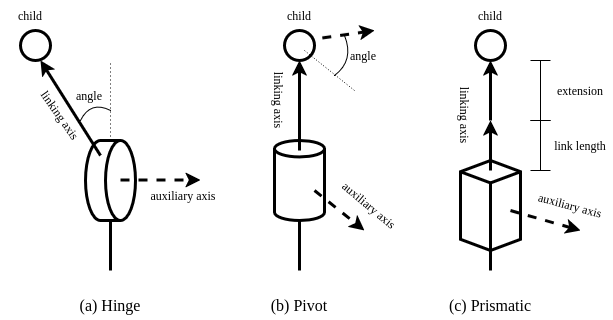
\includegraphics[width=1\textwidth]{graphics/inverse_kinematics/joint_diagrams.png}
    \caption{Illustration of different types of joints}
    \label{fig_ik:joint_types}
\end{figure}

\begin{table}[h!]
\centering
\caption{Joint members}
\label{tab_ik:joint_members}
\small{
\begin{tabular}{|l|l|p{0.5\linewidth}|}
    \hline
    \textbf{Member Name} & \textbf{Type} & \textbf{Description} \\
    \hline \hline
    \verb|joint_type| & Enum & The type of motion this joint is limited to, such as "Hinge" \\
    \hline
    \verb|len_link| & Float & Fixed distance from this joint to its child\footnotemark[1] \\
    \hline
    \verb|pos| & Vector3 & Absolute position in space \\
    \hline
    \verb|axis_link| & Vector3 & Unit vector pointing to its child\footnotemark[1], referred to as the Z-axis by Moreno \textit{et al.}\\
    \hline
    \verb|axis_aux| & Vector3 & Perpendicular vector about which a hinge rotates, referred to as the X-axis by Moreno \textit{et al.}\\
    \hline
    \verb|value| & Float & The angle of rotation of a hinge or pivot, or the extension of a prismatic joint \\
    \hline
    \verb|limited| & Boolean & Whether or not the joint's range of motion is limited, hence limiting \verb|value| \\
    \hline
    \verb|min| & Float & The lower bound of the range of motion \\
    \hline
    \verb|max| & Float & The upper bound of the range of motion \\
    \hline
\end{tabular}
}
\end{table}

\footnotetext[1]{In this paper, the "child" of a joint is another joint which is directly attached to and manipulated by it.}

In the adapted FABRIK algorithm, joints always need another joint before and after them, in order to be adjusted during both the forward and backward-reaching phases. This necessitates having dummy joints at the start and end of the array, which behave as the mounting base and target respectively.\\
In this subsystem's implementation, a new "reference" joint type is introduced to resolve this issue. This joint type does not inherently displace subsequent joints. Its behaviour is equivalent to a prismatic joint whose linking-length and extension are fixed at zero.\\
A third instance of this joint type is necessary to model the end-effector. In the case of a serial manipulator with only one functional joint, that joint would simply be thrown back and forth between the base and target, never having its \verb|value| be adjusted towards a solution. This is because a joint's \verb|value| is only ever adjusted when a neighbouring joint is moved, and that movement is dependent on it. This is resolved by adding another reference joint before the target joint, which will undergo the FABRIK process.

\newpage
\begin{algorithm}[h!]
\caption{FABRIK Algorithm}
\label{alg:fabrik}
\normalsize{
\begin{algorithmic}[1]
    \Require An array $J$ of joints where $J[0]$ is the base, $J[n-2]$ is the end-effector, and $J[n-1]$ is the target, an acceptable squared error $e$, and a maximum number of forward-backward iterations $m$
    \Ensure The end-effector is within $e$ of the target, or iterations reach maximum
    
    \Function{Fabrik}{$J,e,m$}
        \LineComment[0]{Loop until error reduced or iterations maxed}
        \State $error\gets |J[n-1].\vec{pos}-J[n-2].\vec{pos}|^2$
        \State $error\gets error+|J[n-1].\vec{axis}_{link}-J[n-2].\vec{axis}_{link}|^2$
        \State $error\gets error+|J[n-1].\vec{axis}_{aux}-J[n-2].\vec{axis}_{aux}|^2$
        \State $i\gets 0$
        \While{$i<m$ \textbf{and} $error>e$}
            \LineComment[1]{Forward reaching}
            \For{$j\gets (n-2)\text{ to }1$}
                \If {$J[j+1]$ is a reference}
                    \State $\text{ForwardReference}(J, j)$
                \ElsIf {$J[j+1]$ is a hinge}
                    \State $\text{ForwardHinge}(J, j)$
                \ElsIf {$J[j+1]$ is a pivot}
                    \State $\text{ForwardPivot}(J, j)$
                \ElsIf {$J[j+1]$ is prismatic}
                    \State $\text{ForwardPrismatic}(J, j)$
                \EndIf
            \EndFor
            \Statex

            \LineComment[1]{Backward reaching}
            \For{$j\gets 1\text{ to }(n-2)$}
                \If {$J[j-1]$ is a reference}
                    \State $\text{BackwardReference}(J, j)$
                \ElsIf {$J[j-1]$ is a hinge}
                    \State $\text{BackwardHinge}(J, j)$
                \ElsIf {$J[j-1]$ is a pivot}
                    \State $\text{BackwardPivot}(J, j)$
                \ElsIf {$J[j-1]$ is prismatic}
                    \State $\text{BackwardPrismatic}(J, j)$
                \EndIf
            \EndFor
            \Statex

            \LineComment[1]{End iteration}
            \State $error\gets |J[n-1].\vec{pos}-J[n-2].\vec{pos}|^2$
            \State $error\gets error+|J[n-1].\vec{axis}_{link}-J[n-2].\vec{axis}_{link}|^2$
            \State $error\gets error+|J[n-1].\vec{axis}_{aux}-J[n-2].\vec{axis}_{aux}|^2$
            \State $i\gets i+1$
        \EndWhile
    \EndFunction
\end{algorithmic}
}
\end{algorithm}

\newpage
Moreno \textit{et al.} don't consider an edge-case in their adapted FABRIK algorithm, in which the last functional joint is a pivot. This case is relevant to the Braccio, as its wrist joint is modelled by a pivot. During the backwards-reaching phase of such a scenario, the auxiliary axis of the end-effector would be chosen such that, if it were a hinge, it would more easily accommodate for its child. This assumption doesn't hold for such a case and leads to less desirable results. This subsystem instead handles this case uniquely, and chooses an auxiliary axis that best aligns with the target's auxiliary axis. It does so by projecting the target's auxiliary axis onto the plane defined by the pivot's linking axis, and all subsequent processing is identical to the original algorithm; check for zero magnitude, normalise, and apply bounds on range of motion.

\section{Implementation for the Braccio}
The Braccio was modelled as having five functional joints, and hence an array of eight Joint structs (to include the base, end-effector, and target). The configuration for each joint is shown in \autoref{tab_ik:braccio_config}. The shoulder joint's range of motion was confined to 0 degrees, aligning with the 2D dimensional restriction discussed in \autoref{sec_comp_vis:target_generation}. This makes the joint redundant, but it was kept for the sake of being more explicit, and deemed to have negligible effect on the overall performance of the system.

Each time an inverse kinematics solution needs to be found, the target position, direction, and rotation from the computer vision subsystem is parsed as the target position, linking axis, and auxiliary axis, respectively. The auxiliary axis is then projected onto the plane defined by the linking axis and normalised again, to ensure that it's perpendicular to the linking axis. In edge cases with zero magnitude, the previous inverse kinematics solution is returned. After setting the target, the adapted FABRIK algorithm is run, starting at the previous solution, for up to 10,000 iterations while aiming for a squared error under 1mm$^2$. The 10,000 iteration limit was experimentally selected by testing the computation time for different limits in scenarios that struggled to converge. The solver returns the \verb|value|s of the functional joints, which then all undergo a mapping to the Braccio's native angular measurements, giving five setpoints.

Considering the computationally heavy nature of a numerical process, the algorithm was implemented in Rust (1.99.0) as opposed to Python. The Maturin (1.15.0) package was used to compile the Rust code into a Python module, giving the Python main loop access to inverse kinematics function calls and return values. This subsystem was run on the same laptop described in \autoref{tab_comp_vis:laptop_specs}.

\begin{table}[h!]
\centering
\caption{Braccio joint configurations}
\label{tab_ik:braccio_config}
\small{
\begin{tabular}{|l|c|c|c|c|c|c|c|c|}
    \hline
    \textbf{Member} & \textbf{Base} & \textbf{Shoulder} & \textbf{Arm 1} & \textbf{Arm 2} & \textbf{Arm 3} & \textbf{Wrist} & \textbf{EE} & \textbf{Target} \\
    \hline \hline
    \verb|joint_type| & Reference & Pivot & Hinge & Hinge & Hinge & Pivot & Reference & Reference \\
    \hline
    \verb|len_link| & N/A & 68mm & 123mm & 123mm & 62mm & 125mm & N/A & N/A \\
    \hline
    \verb|pos| & 0, 0, 3mm & - & - & - & - & - & - & position \\
    \hline
    \verb|axis_link| & 0, 0, 1mm & - & - & - & - & - & - & direction \\
    \hline
    \verb|axis_aux| & 1mm, 0, 0 & - & - & - & - & - & - & rotation \\
    \hline
    \verb|value| & N/A & - & - & - & - & - & N/A & N/A \\
    \hline
    \verb|limited| & N/A & true & true & true & true & true & N/A & N/A \\
    \hline
    \verb|min| & N/A & 0\degree & -75\degree & -90\degree & -90\degree & -90\degree & N/A & N/A \\
    \hline
    \verb|max| & N/A & 0\degree & 75\degree & 90\degree & 90\degree & 90\degree & N/A & N/A \\
    \hline
\end{tabular}
}
\end{table}

\newpage
\section{Testing}\label{sec_ik:testing}

\subsection{Acceptance Test Procedures}\label{ssec_ik:ATPs}
The inverse kinematics solver is acceptance-tested in isolation from the Braccio-specific implementation of the subsystem. Each of the main three joint types undergo three scenarios in which they are the only joint of a serial manipulator (1 degree of freedom):
\begin{enumerate}[nosep]
    \item The joint's range of motion is not constrained, and the target is perfectly reachable.
    \item The joint's range of motion is not constrained, but the target is unreachable regardless, due to the kinematics of the joint.
    \item The joint's range of motion is constrained, and the target would be reachable if not for the constrain.
\end{enumerate}

This creates a total of nine ATPs. Each ATP is given up to 100 iterations, aiming for less than 1mm$^2$ of error. An ATP is passed if the returned solution (\verb|value| associated with the Joint) is within 0.01 degrees or millimetres of the expected solution. The exact set of scenarios used to test the inverse kinematics solver can be found in \autoref{app:D_ik_ATPs}.

\subsection{Benchmarking}
This subsystem is benchmarked on the time taken to attempt to find an inverse kinematics solution, the number of iterations in attempts, and the remaining error after attempts. Time is measured using the \verb|monotonic()| function from the \verb|time| module in Python. The total error encompasses the error in the position, direction and rotation, in a sum-of-squares relationship.

Data was generated during the same teleoperation task used to generate data for the computer vision subsystem. A video of this task can be found on \href{https://github.com/Neo-Vorsatz-UCT/eee4022s/blob/main/data/EEE4022S_TDR-04_Demo.mp4}{GitHub}.
